\documentclass[asp1.tex]{subfiles}
\begin{document}
\section{(No-)SQL - Datenbanken}
\subsection{Unterschied NoSQL vs. SQL}
Einfach gesagt ist \textbf{SQL} eine Sprache um Abfragen auf relationale Datenbanken zu machen. \\
\textbf{NoSQL} Datenbanken brauchen keine Abfragesprache (Query Language) um benutzt zu werden, da die Daten nicht in Relationen gespeichert werden. \\
In den meisten Fällen werden relationale Datenbanken benötigt. Wenn Daten jedoch unstrukturiert oder nur als Key-Value-Paar gespeichert werden, wird zu NoSQL-Datenbanken geraten, da diese schneller sind.

\subsection{Was ist eine Datenbank?}

Eine Datenbank, auch Datenbanksystem (DBS) genannt, ist ein System zur elektronischen Datenverwaltung. \\ \\
Die wesentliche Aufgabe eines DBS ist es, große Datenmengen
\begin{itemize}
    \item Effizient
    \item Widerspruchsfrei
    \item Dauerhaft
\end{itemize}
zu speichern.

\subsection{Wie ist eine Datenbank aufgebaut?}
Eine Datenbank besteht aus zwei Teilen: \\
\begin{enumerate}
    \item Verwaltungssoftware, genannt Datenbankmanagementsystem (DBMS) \\
          \begin{itemize}
              \item Organisiert intern die strukturierte Speicherung der Daten
              \item Kontrolliert alle lesenden und schreibenden Zugriffe auf die Datenbank
          \end{itemize}
    \item Der Menge der zu verwaltenden Daten
\end{enumerate}

\subsection{Was ist ein Datenbankmanagementsystem (DBMS)?}
Ein relationales Datenbankmanagementsystem besteht aus Tabellen (Relationen), die untereinander in Beziehung (Kardinalität) stehen. \\
z.B.: Lieferanten- und Artikeldaten stehen in separaten Tabellen, die Beziehung gibt an welcher Lieferant welche Artikel liefert.

\subsection{SQL}

SQL ist eine Programmiersprache, mit der man Abfragen auf relationale Datenbanken ausführt.

\subsubsection{Basics (SELECT, FROM)}
Die Einfachste Abfrage benötigt 2 Schlüsselwörter:
\begin{itemize}
    \item SELECT - bestimmt die Felder, die am Ende dargestellt werden sollen
    \item FROM - bestimmt die Datenbanken, die abgefragt werden sollen \\
\end{itemize}
Will man die Namen der Schüler einer Schule ausgeben könnte der Befehl wie folgt aussehen:
\begin{lstlisting}
SELECT vorname,  nachname
FROM SCHUELER
\end{lstlisting}
\begin{verbatim}
Micha Schmitt
Shanine Gmyrek
Ole Lorbacher
Gerhard Benkovsky
\end{verbatim}

\subsubsection{WHERE}
Mit der \textbf{WHERE}-Klausel kann man die Suche weiter einschränken:
\begin{lstlisting}
SELECT *
FROM SCHUELER
WHERE company = `SAP`
\end{lstlisting}
\begin{verbatim}
Micha Schmitt  19  E2FI1 SAP
\end{verbatim}
Es ist möglich, mehrere Bedingungen anzugeben. \\
Dazu  benutzt man \textbf{AND} und \textbf{OR}.\\
Zudem kann eine Bedingung mit \textbf{NOT} verneint  werden.
\begin{lstlisting}
SELECT *
FROM SCHUELER
WHERE company = `SAP`  AND NOT age > 18  OR  name LIKE M%
\end{lstlisting}

\subsubsection{Wildcard}
Will man alle Felder, kann man eine \textbf{Wildcard} benutzen:
\begin{lstlisting}
SELECT * FROM SCHUELER
\end{lstlisting}
\begin{verbatim}
Micha Schmitt  19  E2FI1 SAP
...
\end{verbatim}
Ein \_ steht  für  ein einzelnes Zeichen.
\begin{lstlisting}
SELECT *
FROM SCHUELER
WHERE NAME LIKE sch_f
\end{lstlisting}
Hier würde `schaf` gefunden werden,  jedoch nicht `schaffen` \\
\textbf{Note}: Es gibt noch weitere Wildcards, jedoch  sind diese zu spezifisch für die ASP 1.

\subsubsection{Etwas ausdrücklich als Text kennzeichnen}

Falls ein Tabellenname auch gleichzeitig ein Keyword ist, kann SQL die Abfrage nicht ausführen. \\
Um SQL zu sagen, dass es sich um Text handelt (z.B.. Tabellen-Name), benutzt man ´\textless Keyword\textgreater´

\begin{lstlisting}
CREATE TABLE <name>
(
name varchar(255)
`alter` int
)
\end{lstlisting}

\subsubsection{Alias}
Haben Tabellen zu lange oder gleiche Namen, so hilft es oft ihnen \textbf{Aliase} zu geben.
\begin{lstlisting}
SELECT name
FROM SCHUELER AS S
\end{lstlisting}
In diesem Beispiel wäre S.name das Feld name der Tabelle S (Schueler).

\subsubsection{Subqueries}
Mit \textbf{Subqueries} können die Abfragen noch komplexer werden.
\begin{lstlisting}
SELECT *
FROM SCHUELER
WHERE age = (
SELECT MAX(age) FROM SCHUELER
) AS aeltester
\end{lstlisting}
Dieses Beispiel gibt die ältesten Schüler aus. \\
Zudem heißt das Ergebnis  der Subquery `aeltester'.

\subsubsection{Aggregatfunktionen, GROUP BY, HAVING}

Man kann die gefundenen Daten auch in Gruppen einteilen und dann auf diese Gruppen weitere Abfragen machen.
\begin{lstlisting}
SELECT ort, COUNT(name)
FROM CUSTOMER
GROUP BY ort
\end{lstlisting}
In diesem Beispiel werden die Kunden nach ihrem Ort gruppiert. \\
Danach wird der Ort mit der Anzahl aller Kunden ausgegeben. \\
Dabei werden doppelte Namen ignoriert
Um Gruppen  auf bestimme  Bedingungen zu prüfen wird das \textbf{HAVING}-Keyword benutzt. \\

\break

\begin{lstlisting}
SELECT column_name(s)
FROM table_name
WHERE condition
GROUP BY column_name(s)
HAVING condition
ORDER BY column_name(s);
\end{lstlisting}
Neben dem Count gibt es noch weitere Aggregatfunktionen. \\
\begin{itemize}
    \item COUNT
    \item MAX
    \item MIN
    \item AVG
    \item SUM
\end{itemize}

\subsubsection{SELECT DISTINCT}
Es kann vorkommen, dass bei der Ausgabe doppelte Werte ignoriert werden sollen. \\
z.B. wenn man  alle Länder wissen will, in denen man Kunden hat.
\begin{lstlisting}
SELECT DISTINCT country
FROM customers
\end{lstlisting}
\subsubsection{DATABASE}

Mit dem Befehl
\begin{lstlisting}
CREATE DATABASE <Name>
\end{lstlisting}
wird eine Datenbank erstellt.
Mit dem Befehl
\begin{lstlisting}
DROP DATABASE <Name>
\end{lstlisting}
kann man sie wieder löschen.
\subsubsection{CREATE TABLE}

Mit dem Befehl
\begin{lstlisting}
CREATE TABLE <name>
(
name varchar(255)
`alter` int
)
\end{lstlisting}
wird eine Tabelle erstellt. \\ \\

\break

Mit dem Befehl
\begin{lstlisting}
DROP TABLE <Name>
\end{lstlisting}
wird eine  Tabelle gelöscht. \\ \\
Um ein Feld als Primary Key oder Foreign Key zu kennzeichnen verwendet man folgenden Code:
\begin{lstlisting}
CREATE TABLE <name>
(
name varchar(255)
id int NOT NULL AUTO_INCREMENT
`alter` int
PRIMARY KEY(name),
FOREIGN KEY(fieldName) REFERENCES otherTableName(fieldName)
)
\end{lstlisting}
das Feld `id` ist zudem gekennzeichnet, dass es nicht null sein darf. \\
Zudem übergibt man den Wert des Feldes nicht manuell sondern er wird automatisch vom DBMS erstellt.
\subsubsection{INSERT INTO}
Um Daten in die Tabelle einzufügen kann man so vorgehen:
\begin{lstlisting}
INSERT INTO <tabellenName> (name, alter)
VALUES
(Micha,  19),
(Shanine, 18)
\end{lstlisting}
In diesem Beispiel werden zu Einträge in die Tabelle hinzugefügt

\subsubsection{ALTER TABLE}
Um die Struktur einer Tabelle  im Nachhinein noch  zu  verändern  benutzt  man den ALTER-Befehl.
\begin{lstlisting}
ALTER TABLE <tableName>
ADD PLZ char(5)
\end{lstlisting}
Dieser Befehl  würde  eine Spalte  namens  PLZ  hinzufügen.

\subsubsection{UPDATE .. SET ..}

Mit dem UPDATE-Befehl kann man Inhalte der Tabelle überschreiben
\begin{lstlisting}
UPDATE <tableName> SET ekPreis = ekPreis + (ekPreis * 0.02)
\end{lstlisting}
In diesem Beispiel wird die Spalte ekPreis auf das 1,02-fache des ursprünglichen Wertes gesetzt

\subsubsection{DELETE}
Um Daten zu löschen benutzt man den \textbf{DELETE}-Befehl
\begin{lstlisting}
DELETE *
FROM artikel
WHERE VkPreis < 2;
\end{lstlisting}

\subsubsection{ORDER BY}
Um die Ergebnisse einer Abfrage zu sortieren kann man den \textbf{ORDER BY}-Befehl  benutzen.
\begin{lstlisting}
SELECT ArtikelNr, Bezeichnung, Bestand
FROM Artikel
ORDER BY ArtikelNr ASC
\end{lstlisting}
Neben ASC (aufsteigend)  gibt es noch DESC (absteigend)

\subsubsection{LIMIT}
Mit dem \textbf{LIMIT} Keyword kann man die Anzahl der Ergebnisse begrenzen.
\begin{lstlisting}
SELECT ArtikelNr, Bezeichnung, Bestand
FROM Artikel
ORDER BY ArtikelNr ASC
LIMIT 1
\end{lstlisting}
In diesem  Beispiel wird der Eintrag mit der kleinsten Artikelnummer ausgegeben. \\
Der 1. Eintrag  ist der  Kleinste  und alle danach werden aufgrund des \textbf{LIMIT} ignoriert.

\subsubsection{LIKE}
Um nach Text in einem Ergebnis zu filtern wird das \textbf{LIKE}-Keyword benutzt.
\begin{lstlisting}
SELECT * FROM Product
WHERE name LIKE 'Stahl%';
\end{lstlisting}
Hier wird gefiltert,  ob ein Name mit  `Stahl` beginnt.

\subsubsection{ADD CONSTRAINT}
Um eine Verbindung zwischen 2 Tabellen zu zeigen, benutzt man sogenannte Constraints
\begin{lstlisting}
ALTER TABLE `artikel`
ADD CONSTRAINT `FK_artikel_kreditor`
FOREIGN KEY (`LiefNr`) REFERENCES `kreditor` (`LiefNr`)
\end{lstlisting}
In diesem Beispiel wird für die Tabelle `Artikel` eine Verbindung zur Tabelle `kreditor` gemacht. \\
Die Spalte LiefNr von Artikel ist nun der FK für den PK (LiefNr) der Tabelle kreditor.

\subsubsection{JOINS}
Mit Joins kann  man die  Inhalte zweier Tabellen  kombinieren. \\
Die JOIN-Varianten können unten eingesehen werden. \\
Es gibt noch mehr JOINS, jedoch werden diese sehr sehr unwahrscheinlich in einer ASP 1 drankommen.
\begin{figure}[H]
    \begin{center}
        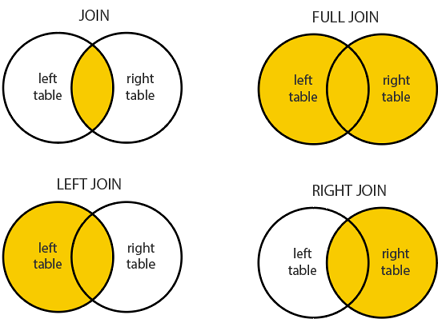
\includegraphics[height=6cm]{joins.png}
    \end{center}
    \caption{The Types of JOINs}
    \label{fig:types of joins}
\end{figure}
\begin{lstlisting}
SELECT column_name(s)
FROM table1
LEFT JOIN table2
ON table1.column_name = table2.column_name;
\end{lstlisting}

\subsection{Normalisierung von Datenbanken}

Unter Normalisierung eines relationalen Datenschemas (Tabellenstruktur) versteht man die Aufteilung von Attributen (Tabellenspalten) in mehrere Relationen (Tabellen) gemäß den Normalisierungsregeln, sodass eine Form entsteht, die keine vermeidbaren Redundanzen mehr enthält.

\subsubsection{1. Normalform}

Eine Relation befindet sich in der ersten Normalform, wenn alle Attribute nur einfache Attributwerte aufweisen (Bezeichnung: atomar)

\subsubsection{2. Normalform}

Eine Relation befindet sich in der zweiten Normalform, wenn sie in der ersten Normalform ist und jedes Nichtschlüsselattribut vom Primärschlüssel voll funktional abhängig ist.

\subsubsection{3. Normalform}

Eine Relation befindet sich in der dritten Normalform, wenn sie in der zweiten Normalform ist und jedes Nichtschlüsselattribut nicht transitiv vom Primärschlüssel abhängig ist, d.h. aus keinem Nichtschlüsselattribut folgt ein anderes Nichtschlüsselattribut.



\subsubsection{Beispiel}

\textbf{Ausgangstabelle}
\begin{table}[H]
    \centering
    \begin{tabular}{|p{0.2\textwidth}|p{0.2\textwidth}|p{0.2\textwidth}|p{0.2\textwidth}|p{0.2\textwidth}|}
        \hline
        CD\textunderscore ID & Album                           & Gründungsjahr & Erscheinungsjahr & Titelliste                                                \\\hline

        4711                 & Anastacia – Not That Kind       & 1999          & 2000             & (1. Not That Kind, 2. I’m Otta Love, 3. Cowboys \& Kisses \\\hline

        4712                 & Pink Floyd – Wish You Were Here & 1965          & 1975             & (1. Shine On You Crazy Diamond)                           \\\hline

        4713                 & Anastacia – Freak of Nature     & 1999          & 2002             & (1. Paid my Dues)
        \\\hline
    \end{tabular}
\end{table}

\textbf{1. Normalform}
\begin{table}[H]
    \centering
    \begin{tabular}{|p{0.1\textwidth}|p{0.1\textwidth}|p{0.1\textwidth}|p{0.2\textwidth}|p{0.2\textwidth}|p{0.1\textwidth}|p{0.1\textwidth}|}
        \hline

        CD\textunderscore ID & Albumtitel         & Interpret  & Gründungsjahr & Erscheinungsjahr & Track & Titel                      \\\hline

        4711                 & Not That Kind      & Anastacia  & 1999          & 2000             & 1     & Not That Kind              \\\hline

        4711                 & Not That Kind      & Anastacia  & 1999          & 2000             & 2     & I’m Outta Love             \\\hline

        4711                 & Not That Kind      & Anastacia  & 1999          & 2000             & 3     & Cowboys \& Kisses          \\\hline

        4712                 & Wish You Were Here & Pink Floyd & 1965          & 1975             & 1     & Shine On You Crazy Diamond \\\hline

        4713                 & Freak of Nature    & Anastacia  & 1999          & 2002             & 1     & Paid my Dues

        \\\hline
    \end{tabular}
\end{table}


\textbf{2. Normalform}
\begin{table}[H]
    \centering
    \begin{tabular}{|p{0.2\textwidth}|p{0.2\textwidth}|p{0.2\textwidth}|p{0.2\textwidth}|p{0.2\textwidth}|}
        \hline
        CD\textunderscore ID & Albumtitel         & Interpret  & Gründungsjahr & Erscheinungsjahr \\\hline

        4711                 & Not That Kind      & Anastacia  & 2000          & 2000             \\\hline

        4712                 & Wish You Were Here & Pink Floyd & 1975          & 1975             \\\hline

        4713                 & Freak of Nature    & Anastacia  & 2002          & 2001

        \\\hline
    \end{tabular}
    \caption{CD}
\end{table}

\begin{table}[H]
    \centering
    \begin{tabular}{|p{0.3\textwidth}|p{0.3\textwidth}|p{0.3\textwidth}|}
        \hline
        CD\textunderscore ID & Track & Titel                      \\\hline

        4711                 & 1     & Not That Kind              \\\hline

        4711                 & 2     & I’m Outta Love             \\\hline

        4711                 & 3     & Cowboys \& Kisses          \\\hline

        4712                 & 1     & Shine On You Crazy Diamond \\\hline

        4713                 & 1     & Paid my Dues

        \\\hline
    \end{tabular}
    \caption{Lied}
\end{table}

\break
\textbf{3. Normalform}
\begin{table}[H]
    \centering
    \begin{tabular}{|p{0.25\textwidth}|p{0.25\textwidth}|p{0.25\textwidth}|p{0.25\textwidth}|}
        \hline

        CD\textunderscore ID & Albumtitel         & Interpret\textunderscore ID & Erscheinungsjahr \\\hline

        4711                 & Not That Kind      & 311                         & 2000             \\\hline

        4712                 & Wish You Were Here & 312                         & 1975             \\\hline

        4713                 & Freak of Nature    & 311                         & 2001

        \\\hline
    \end{tabular}
    \caption{CD}
\end{table}

\begin{table}[H]
    \centering
    \begin{tabular}{|p{0.25\textwidth}|p{0.25\textwidth}|p{0.25\textwidth}|}
        \hline

        Interpret\textunderscore ID & Interpret  & Gründungsjahr \\\hline

        311                         & Anastacia  & 1999          \\\hline

        312                         & Pink Floyd & 1965

        \\\hline
    \end{tabular}
    \caption{Künstler}
\end{table}

\begin{table}[H]
    \centering
    \begin{tabular}{|p{0.25\textwidth}|p{0.25\textwidth}|p{0.25\textwidth}|}
        \hline

        CD\textunderscore ID & Track & Titel                      \\\hline

        4711                 & 1     & Not That Kind              \\\hline

        4711                 & 2     & I’m Outta Love             \\\hline

        4711                 & 3     & Cowboys \& Kisses          \\\hline

        4712                 & 1     & Shine On You Crazy Diamond \\\hline

        4713                 & 1     & Paid my Dues

        \\\hline
    \end{tabular}
    \caption{Lied}
\end{table}

Anmerkung: Wenn Interpret weltweit eindeutig wäre, wäre der künstliche Schlüssel ‚Interpret\textunderscore ID‘ nicht zwingend notwendig.


\subsection{Rechte- und Benutzerverwaltung - vermutlich nicht ASP1}

Mit Hilfe von SQL können Benutzer und Rechte angelegt und verteilt werden. Ein fein unterteiltes Rechtesystem hilft dabei, die Zugriffsberechtigungen von unterschiedlichen Nutzern zu steuern.

\subsubsection{Anlegen von Benutzern}

\begin{lstlisting}
CREATE USER `bob` identified by `test`
\end{lstlisting}
\begin{itemize}[topsep=-10pt]
    \item Legt einen Benutzer bob mit dem Passwort test an
    \item Benutzer kann von überall her auf die Datenbank zugreifen
\end{itemize}

\vspace{20pt}
\begin{lstlisting}
    CREATE USER `tom` identified by `test` WITH MAX_QUERIES_PER_HOUR 2000 PASSWORD EXPIRE INTERVAL 90 DAY;
\end{lstlisting}
\begin{itemize}[topsep=-10pt]
    \item Legt einen Benutzer tom mit dem Passwort test an
    \item Benutzer kann von überall her auf die Datenbank zugreifen
    \item Maximal 2000 Anfragen pro Stunde
    \item Passwort muss spätestens nach 90 Tagen erneuert werden
\end{itemize}

\subsubsection{Zuweisen von Rechten}
\begin{lstlisting}
    GRANT ALL ON haro02.* TO bob
    FLUSH PRIVILEGES
\end{lstlisting}
\begin{itemize}[topsep=-10pt]
    \item GRANT ALL PRIVILEGES: Alle Verfügbaren Rechte werden vergeben (Rechte können fein granuliert werden \textrightarrow\space \url{https://mariadb.com/kb/en/grant/}
    \item Benutzer kann von überall her auf die Datenbank zugreifen
    \item Maximal 2000 Anfragen pro Stunde
    \item Passwort muss spätestens nach 90 Tagen erneuert werden
\end{itemize}

\subsubsection{Anzeigen aller Benutzer}
\begin{lstlisting}
    SELECT * FROM mysql.user
\end{lstlisting}

\subsubsection{Benutzer löschen}
\begin{lstlisting}
    DROP USER bob
\end{lstlisting}


\subsection{Transaktionsverwaltung - vermutlich nicht ASP1}
Unter einer DB-Transaktion versteht man eine Sammlung von Befehlen, die als logische Einheit verstanden werden.
Entweder sind alle Befehle erfolgreich oder keiner.
Fehlerhafte Transaktionen müssen abgebrochen werden und bisherige Änderungen in der Datenbank rückgängig gemacht werden.

\subsubsection{ACID-Prinzip}
Beim Ausführen einer Transaktion muss das Transaktionssystem die ACID-Eigenschaften garantieren.

\begin{outline}
    \1 Atomarität (Atomicity)
    \2 Transaktion wird entweder ganz oder gar nicht ausgeführt
    \2 Transaktionen sind unteilbar
    \2 Wenn eine atomare Transaktion abgebrochen wird, ist das System unverändert
    \1 Konsistenz (Consisentcy)
    \2 Nach Ausführung einer Transaktion muss der Datenbestand in einer konsistenten Form sein, wenn er es bei Beginn der Transaktion auch schon war
    \1 Isolation (Isolation)
    \2 Bei Ausführung mehrerer Transaktionen gleichzeitig, dürfen diese sich nicht gegenseitig beeinflussen
    \1 Dauerhaftigkeit (Durability)
    \2 Auswirkungen einer Transaktion müssen im Datenbestand dauerhaft bestehen bleiben
    \2 Effekte von Transaktionen dürfen nicht verloren gehen oder verblassen
    \2 Verschachtelung von Transaktionen ist daher streng genommen nicht möglich, da ein Zurücksetzen (Rollback) der äußeren Transaktion die Dauerhaftigkeit der inneren, bereits ausgeführten, Transaktion verletzen würde
\end{outline}

\subsubsection{Ausführen von Transaktionen}

Transaktionen werden durch die Markierungen \textbf{START TRANSACTION} und \textbf{END OF TRANSACTION} (oder \textbf{COMMIT}) abgegrenzt:

\begin{lstlisting}
    START OF TRANSACTION
    WRITE x
    WRITE y
    COMMIT
\end{lstlisting}

\subsubsection{Beenden von Transaktionen}

\begin{enumerate}
    \item Commit: Die Transaktion wurde erfolgreich und ohne Probleme beendet. Die Auswirkungen der Transaktion auf den Datenbestand sind dauerhaft gespeichert.

          Oft werden „COMMIT“ und „END OF TRANSACTION“ synonym verwendet
    \item Rollback: Bei der Ausführung sind Probleme aufgetreten und die Ausführung wird nicht fortgesetzt. Sämtliche Auswirkungen auf den Datenbestand müssen rückgängig gemacht werden (Atomarität).
\end{enumerate}

\subsubsection{Autocommit}

Standardmäßig befindet sich MariaDB im Modus Autocommit. Das bedeutet, dass alle Data Manipulation Befehle direkt persistiert werden.

Autocommit beenden: SET AUTOCOMMIT = 0; dann müssen alle Änderungen am Datenbestand mit COMMIT explizit permanent gespeichert werden.
Mit ROLLBACK werden alle Änderungen bis zum letzten Commit rückgängig gemacht.

Autocommit aktivieren: SET AUTOCOMMIT = 1
\end{document}